\documentclass{standalone}
\usepackage{amsmath,amssymb}
\usepackage[dvipsnames]{xcolor}
\usepackage{tikz} 
\usetikzlibrary{arrows, decorations.markings,decorations.pathreplacing,angles,quotes}
\usepackage{microtype}
\usepackage{fourier}

\definecolor{nb}{rgb}{0.12157, 0.46667, 0.705882}

%include other needed packages here   
\begin{document}

\begin{tikzpicture}
% include your tikz code here
    		\node[anchor=south west,inner sep=0] (Bild) at (0,0) {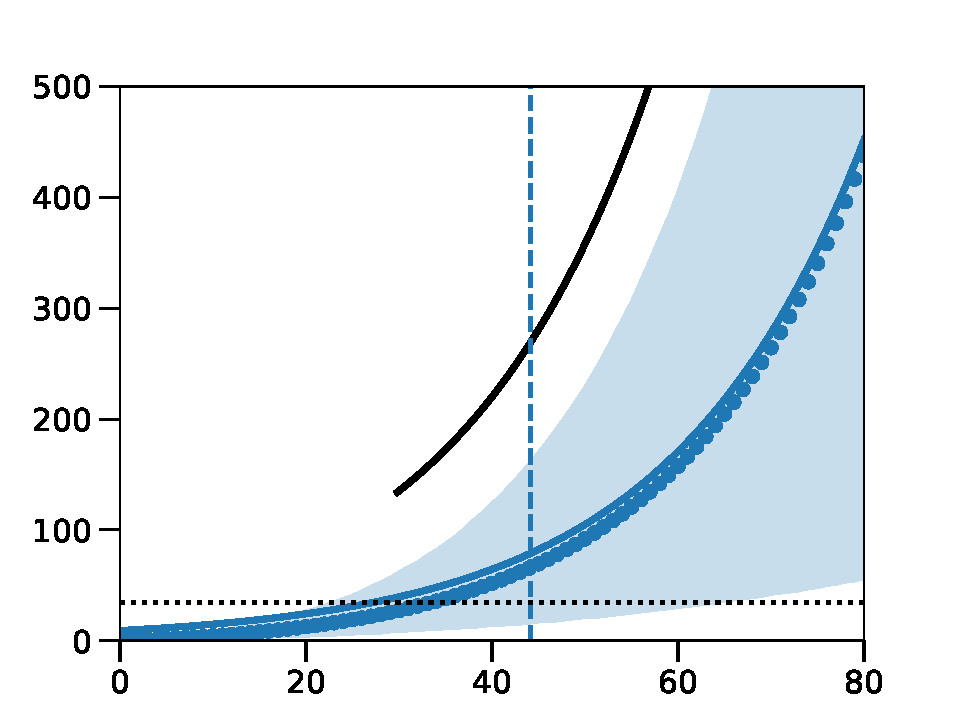
\includegraphics[scale=0.39]{figS4_blank.pdf}};
   		\begin{scope}[x=(Bild.south east),y=(Bild.north west)]
        	\draw (0.55,-0.01) node {time $t$ [days]};
        	\draw (-0.005,0.5) node [rotate=90] {epidemic size at $I_{\text{surv}}(t)$};
        	
        	\draw[color = nb, very thick] (0.925,0.65) -- node[right=6pt] {\color{black} \small Eq. (3)} (0.975,0.65);

        	\draw[color = black, very thick] (0.925,0.77) -- (0.975,0.77);
        	\draw (0.975,0.8) node[right=2pt] {\small improved rule};
        	\draw (0.975,0.74) node[right=2pt] {\small of thumb};
        	
        	\node[right=0pt] at (0.41,0.82) {\small $\widehat{T}_{\text{hosp}}$};
        	
        	\draw[very thick, dotted] (0.925,0.53) -- (0.975,0.53);
        	\node[right=2pt] at (0.975,0.555) {\small Simple rule};
        	\node[right=2pt] at (0.975,.505) {\small rule of thumb};

        	\draw[color = nb] (0.925,0.35) node[right=0pt] {\large $\bullet$};
        	\node[right=2pt] at (0.975,0.38) {\small Simulation};
        	\draw (0.975,0.32) node[right=2pt] {\small averages};

   		\end{scope}
\end{tikzpicture}

\end{document}